% Ferrers diagrams of 6+4+4+2+1 and of its conjugate. Generated by a short script.
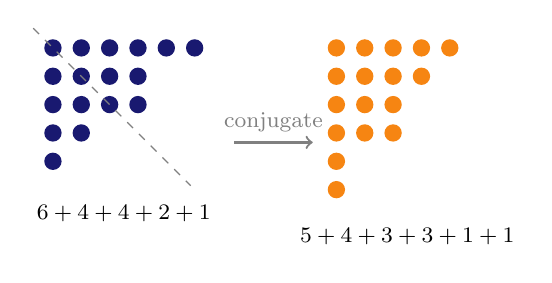
\begin{tikzpicture}[every node/.style={font=\footnotesize}]
\fill[MidnightBlue] (0.000,0.000) circle (0.11);
\fill[MidnightBlue] (0.360,0.000) circle (0.11);
\fill[MidnightBlue] (0.720,0.000) circle (0.11);
\fill[MidnightBlue] (1.080,0.000) circle (0.11);
\fill[MidnightBlue] (1.440,0.000) circle (0.11);
\fill[MidnightBlue] (1.800,0.000) circle (0.11);
\fill[MidnightBlue] (0.000,-0.360) circle (0.11);
\fill[MidnightBlue] (0.360,-0.360) circle (0.11);
\fill[MidnightBlue] (0.720,-0.360) circle (0.11);
\fill[MidnightBlue] (1.080,-0.360) circle (0.11);
\fill[MidnightBlue] (0.000,-0.720) circle (0.11);
\fill[MidnightBlue] (0.360,-0.720) circle (0.11);
\fill[MidnightBlue] (0.720,-0.720) circle (0.11);
\fill[MidnightBlue] (1.080,-0.720) circle (0.11);
\fill[MidnightBlue] (0.000,-1.080) circle (0.11);
\fill[MidnightBlue] (0.360,-1.080) circle (0.11);
\fill[MidnightBlue] (0.000,-1.440) circle (0.11);
\draw[gray,dashed] (-0.25,0.25)--(1.75,-1.75);
\fill[BurntOrange] (3.600,0.000) circle (0.11);
\fill[BurntOrange] (3.960,0.000) circle (0.11);
\fill[BurntOrange] (4.320,0.000) circle (0.11);
\fill[BurntOrange] (4.680,0.000) circle (0.11);
\fill[BurntOrange] (5.040,0.000) circle (0.11);
\fill[BurntOrange] (3.600,-0.360) circle (0.11);
\fill[BurntOrange] (3.960,-0.360) circle (0.11);
\fill[BurntOrange] (4.320,-0.360) circle (0.11);
\fill[BurntOrange] (4.680,-0.360) circle (0.11);
\fill[BurntOrange] (3.600,-0.720) circle (0.11);
\fill[BurntOrange] (3.960,-0.720) circle (0.11);
\fill[BurntOrange] (4.320,-0.720) circle (0.11);
\fill[BurntOrange] (3.600,-1.080) circle (0.11);
\fill[BurntOrange] (3.960,-1.080) circle (0.11);
\fill[BurntOrange] (4.320,-1.080) circle (0.11);
\fill[BurntOrange] (3.600,-1.440) circle (0.11);
\fill[BurntOrange] (3.600,-1.800) circle (0.11);
\node at (0.9,-2.1) {$6+4+4+2+1$};
\node at (4.5,-2.4) {$5+4+3+3+1+1$};
\draw[->,thick,gray] (2.3,-1.2)--(3.3,-1.2) node[midway,above] {conjugate};
\end{tikzpicture}
